\section{Coupled Results}
\label{sec:coupledResults}

\begin{frame}{Remember why we are here}
  \pause
  \huge Model a nuclear reactor.
\end{frame}

\begin{frame}{Advanced Burner Reactor -- MET-1000}
  \begin{itemize}
    \item Benchmark published February 2016 \cite{abr}.
    \item Four designs including MET-1000.
    \item Thirty-one solutions including \dif.
  \end{itemize}
  \vspace{0.2in}
  \begin{itemize}
    \item Eighteen cross-section regions.
    \item Forty-Nine material compositions.
    \item Dimensions and isotopic compositions fully specified.
  \end{itemize}
  \vspace{0.2in}
  \begin{itemize}
    \item Cross-sections generated independently.
    \item Dimensions \textit{appear} thermally expanded.
  \end{itemize}
\end{frame}

\begin{frame}{RESULTS ARE WRONG!}
  \begin{itemize}
    \item This chapter isn't written yet.
    \item I know the results in this section are wrong.
    \item Still working on the model, but I have the scripts to generate these
      plots.
    \item Please look at the ideas, not the numbers.
  \end{itemize}
\end{frame}

\begin{frame}{Reactivity Coefficients}
  Consider a series of reactor powers $P_i = \{0\%,\ldots,100\%\}$. The
  reactivity at power $P_i$ due to feedback can be defined.
  \begin{equation}
    \rho_i = \frac{\keffsub{i} - \keffsub{0}}{\keffsub{i} \, \keffsub{0}}
  \end{equation}
  Define the following reactivity coefficients.
  \begin{align}
    \alpha_{Total} &= \frac{\rho_i(\text{\scriptsize ALL})-
      \rho_0}{P_i} \\
    \alpha_{T_{\!\mbox{\scriptsize \em exp}}} &= \frac{\rho_i(\text{\scriptsize 
      No } T_{\!\mbox{\scriptsize \em exp}} )-
      \rho_0}{P_i} \\
    % (coolant temperature coefficient)
    \alpha_{CTC,i} &= \frac{\rho_i(\text{\scriptsize ALL}) - 
      \rho_i(T_{cool}+\Delta T_{cool})}{\Delta T_{cool}} \\
    \alpha_{Doppler,i} &= \frac{\rho_i(\text{\scriptsize ALL}) - 
      \rho_i(T_{fuel}+\Delta T_{fuel})}{\Delta T_{fuel}}
  \end{align}
\end{frame}

\begin{frame}{Benchmark Result}
  \vspace{-0.25in}
  \begin{figure}
    \centering
    \subfloat[$\phi_{1}$]{
      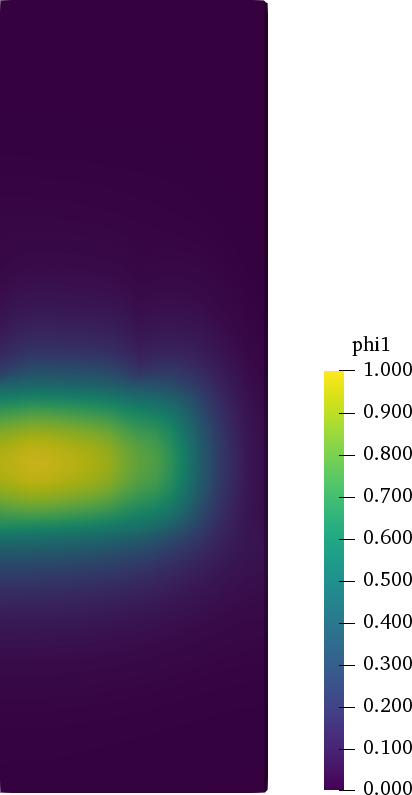
\includegraphics[width=0.25\textwidth]{abr_phi_nod_group1}}
    \hspace{1in}
    \subfloat[$\phi_{33}$]{
      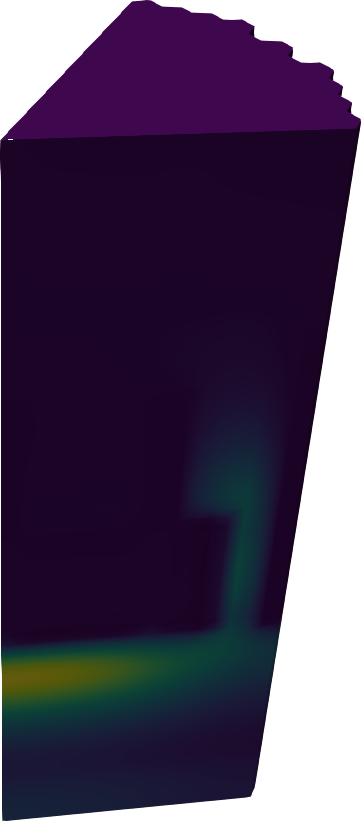
\includegraphics[width=0.25\textwidth]{abr_phi_nod_group33}}
  \end{figure}
  \begin{block}{}
    $\keff =  1.006694 $ \qquad (\dif $-700\units{pcm}$)
  \end{block}
\end{frame}

\begin{frame}{Eigenvalue Feedback}
  \begin{figure}
    \centering
    \includegraphics[width=0.7\textwidth]{keff_feedback}
    \caption{Linear Expansion Factor for HT9 Steel and U10Zr Fuel.}
    \label{fig:lef_plot}
  \end{figure}
\end{frame}

\begin{frame}{Reactivity Coefficients}
  \begin{figure}
    \centering
    \subfloat{
      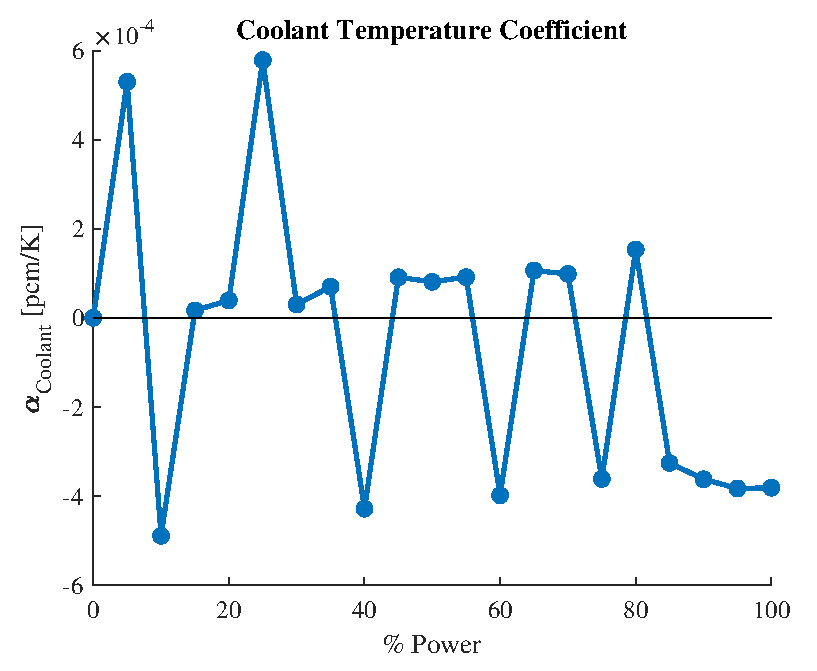
\includegraphics[width=0.5\textwidth]{alpha_ctc}}
    \hspace*{\fill}
    \subfloat{
      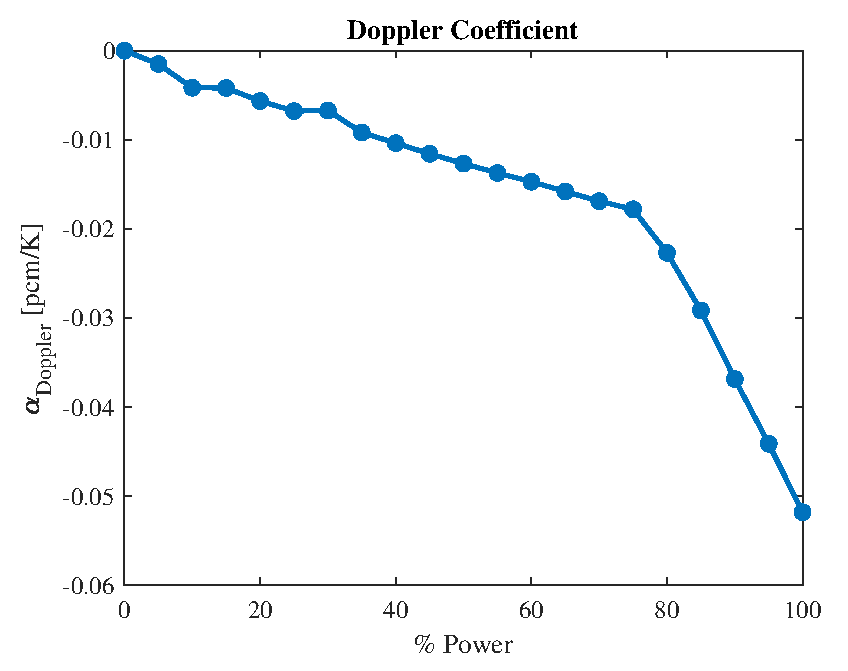
\includegraphics[width=0.5\textwidth]{alpha_doppler}}
  \end{figure}
\end{frame}
